\documentclass[aspectratio=169,10pt]{beamer}
\usetheme{default}
\usecolortheme{default}
\setbeamertemplate{navigation symbols}{}
\setbeamertemplate{footline}[frame number]
\usepackage{booktabs}
\usepackage{graphicx}
\graphicspath{{figures/}}
\definecolor{enh}{HTML}{2A78D6}
\definecolor{base}{HTML}{EB6834}
\setbeamercolor{frametitle}{fg=black}
\setbeamercolor{title}{fg=black}
\setbeamercolor{structure}{fg=enh}
\newcommand{\enh}[1]{\textcolor{enh}{\textbf{#1}}}
\newcommand{\bas}[1]{\textcolor{base}{\textbf{#1}}}

\title{Detecting Meaning Drift in Twitter Sentiment Streams}
\subtitle{Informed ageing naive Bayes + an error-based ADWIN detector,\\on Kafka, Spark, InfluxDB and Grafana}
\author{Group 18 --- \textit{member names}}  % TODO: names
\institute{Streaming Data Analysis, Semester 7}
\date{}

\begin{document}

\begin{frame}
\titlepage
\end{frame}

\begin{frame}{Problem: sentiment streams drift}
\begin{itemize}
\item Tweets are an unbounded stream; topics, vocabulary and opinions change (concept drift).
\item A classifier trained once loses accuracy when real-world events change the discussion
  (Bechini et al., 2021).
\item Two kinds of drift:
  \begin{itemize}
  \item \textbf{virtual}: $P(X)$ changes --- new words, new topics
  \item \textbf{real}: $P(y\,|\,X)$ changes --- the \emph{same} words now mean something else
  \end{itemize}
\item \textbf{Question:} the paper's detector watches the \emph{words}. Does it see changes in
  \emph{meaning}? If not, can watching the model's own \emph{errors} close the gap?
\end{itemize}
\end{frame}

\begin{frame}{Base papers}
\begin{enumerate}
\item \textbf{Iosifidis, Oelschlager, Ntoutsi (2017)} --- informed ageing MNB on Sentiment140:
  forget old counts by $e^{-\lambda \Delta t}$, tune $\lambda$ when a vocabulary detector fires.
  \alert{Our baseline.}
\item \textbf{Costa, Silva, Antunes, Ribeiro (ICMLA 2014)} --- simulate sudden / gradual /
  recurring drift by re-timestamping real tweets. \alert{Our controlled scenarios.}
\item \textbf{Bechini et al.\ (IEEE Access 2021)} --- event-driven drift in a real Twitter stance
  stream. \alert{Our motivation.}
\end{enumerate}
\vspace{1em}
\textbf{Enhancement:} ADWIN (Bifet \& Gavald\`a, 2007) on the prequential 0/1 error stream,
fused with the vocabulary detector.
\end{frame}

\begin{frame}{Baseline: informed ageing MNB}
\begin{columns}[T]
\column{0.52\textwidth}
\begin{itemize}
\item Counts aged \emph{on read}:\\[2pt]
  $P(w\,|\,c) \propto N_{wc}\, e^{-\lambda (t - t^{w,c}_{lo})} + \alpha$, $t$ in \textbf{hours}
\item Vocabulary detector, every $w$ tweets, per class:\\
  $\mathrm{precision} = |V_{\text{window}} \cap V_{\text{ref}}| / |V_{\text{ref}}|$\\
  change if outside $\mu \pm 1.8\sigma$
\item 5 reactions: SlowIncrease\ldots, FastSet\ldots, \textbf{Rebuild}
\end{itemize}
\column{0.46\textwidth}
\small
\textbf{Fixes the paper leaves open}
\begin{itemize}
\item time unit per instance $\Rightarrow$ model forgets in 100 tweets (68\%); per hour works
\item accumulated reference vocabulary $\Rightarrow$ precision drifts down, constant alarms;
  previous window fixes it
\item 10-check history $\Rightarrow$ false alarms; 20 checks
\end{itemize}
\end{columns}
\end{frame}

\begin{frame}{Reproduction matches the paper's ordering}
\centering
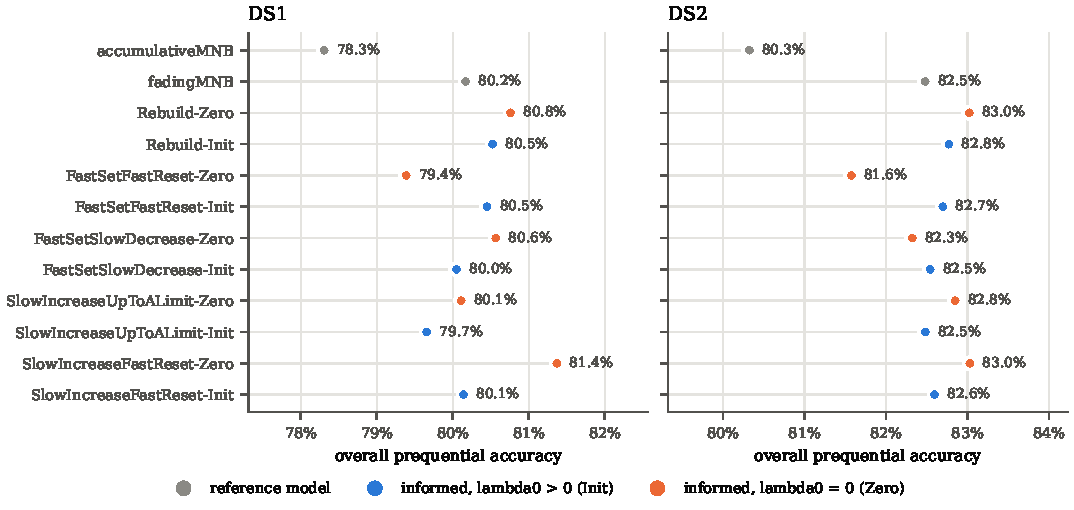
\includegraphics[width=0.92\textwidth]{baseline_overall_accuracy.pdf}\\
\small accumulative worst (78.3 / 80.3\%) $<$ fading $<$ informed (up to 81.4 / 83.0\%);
after DS1's change point adaptive models reach 93--99.9\%.
\end{frame}

\begin{frame}{Enhancement: ADWIN on the prediction error}
\begin{columns}[T]
\column{0.5\textwidth}
\begin{itemize}
\item Prequential: predict, then learn $\Rightarrow$ error $[\hat y \neq y]$ for free
\item ADWIN ($\delta=0.01$): cut when the error rate \textbf{rises}
\item Reaction: \textbf{rebuild on ADWIN's post-drift window}
\item Fusion: adwin\_only, \textbf{OR} (main), AND
\end{itemize}
\column{0.48\textwidth}
\small
\textbf{Learned the hard way}
\begin{itemize}
\item resetting ADWIN after a rebuild blinded it
\item a shared cooldown let one detector's false alarm swallow the other's real alarm
\item padding the rebuild to 1k tweets re-learned the old concept (recovery 5.6k $\to$ 3.0k)
\end{itemize}
\end{columns}
\end{frame}

\begin{frame}{System}
\centering
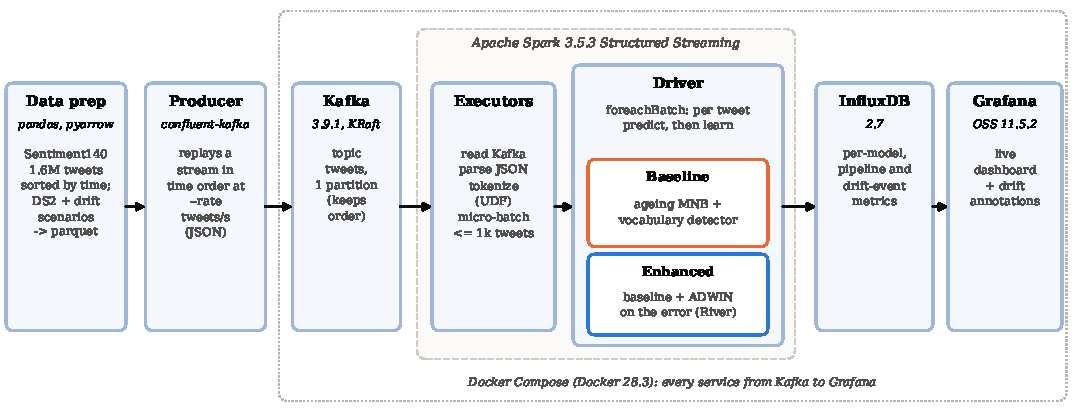
\includegraphics[width=\textwidth]{fig0_architecture.pdf}\\[0.5em]
\small Both models run side by side on identical micro-batches; shared \texttt{core/} package
with the offline runner.
\end{frame}

\begin{frame}{Streams with known drift points}
\begin{itemize}
\item \textbf{DS1}: Sentiment140, 1.6M tweets sorted by time; turns all-negative at 1,324,775
\item \textbf{DS2}: volatile variant, exactly 1,073,065 tweets (paper's counts)
\item \textbf{Scenarios} (80k real tweets, 5 seeds): sudden, gradual, recurring topic switch,
  prior shift 50$\to$10\% positive, \textbf{label flip} (every label inverts, words unchanged),
  \textbf{label flip on one topic}
\item 7 models $\times$ 8 streams = \textbf{224 runs}; metrics: accuracy, P/R/F1, delay, false
  alarms, misses, recovery, cost
\end{itemize}
\end{frame}

\begin{frame}{Headline: label flip (5 seeds)}
\centering
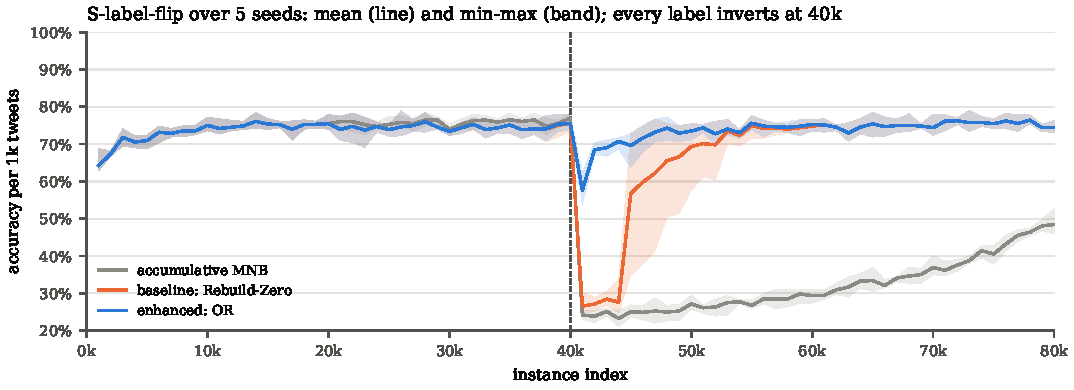
\includegraphics[width=0.95\textwidth]{fig2_label_flip_seeds.pdf}\\
\small
detection \bas{3,999} $\to$ \enh{39} tweets \quad recovery \bas{8,204} $\to$ \enh{3,183}
\quad accuracy \bas{71.0\,$\pm$\,1.0\%} $\to$ \enh{73.8\,$\pm$\,0.3\%}
\end{frame}

\begin{frame}{Detection across all streams}
\centering
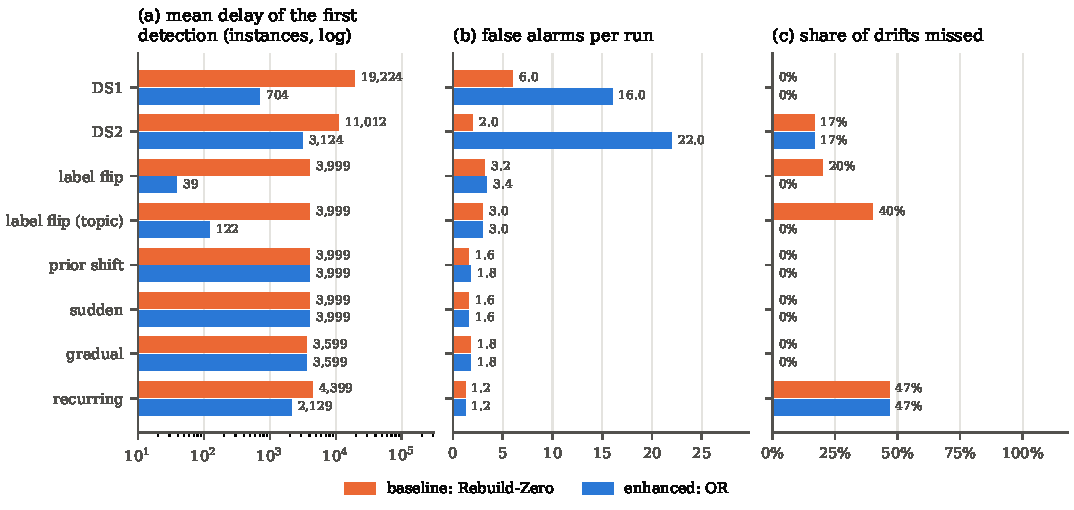
\includegraphics[width=0.95\textwidth]{fig3_detection.pdf}\\
\small topic-only flip: vocabulary detector misses 2 of 5, ADWIN catches 5 of 5 (\textasciitilde120 tweets);
DS1 change point: 19,224 $\to$ 704
\end{frame}

\begin{frame}{Real data and fusion modes}
\centering
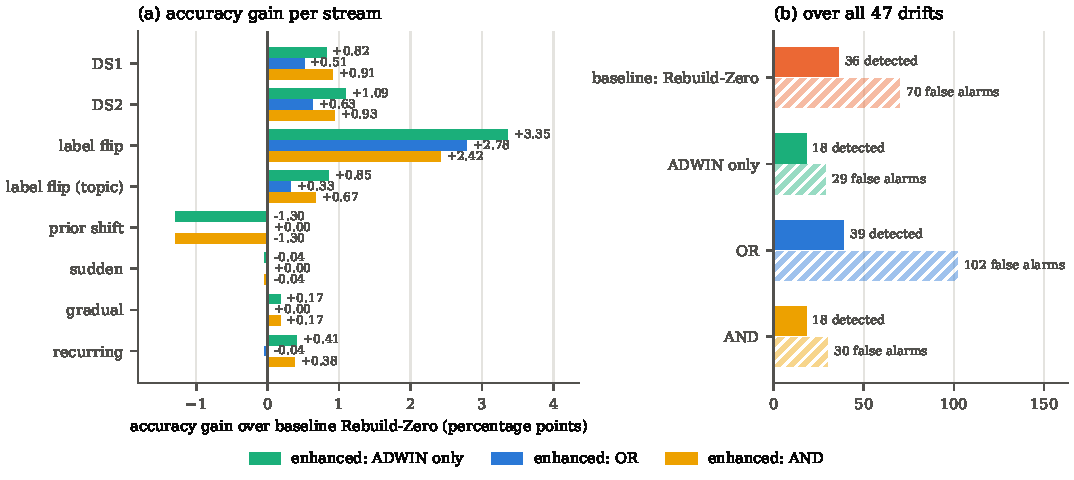
\includegraphics[width=0.9\textwidth]{fig5_ablation.pdf}\\
\small DS1 80.8 $\to$ 81.3--81.7\%, DS2 83.0 $\to$ 83.7--84.1\%. ADWIN misses prior shifts
(no error rise); \textbf{OR} keeps both signals: never $>$0.04 pt below the baseline,
$\geq$ baseline in 28 / 32 stream--seeds.
\end{frame}

\begin{frame}{Live system and cost}
\begin{columns}[T]
\column{0.56\textwidth}
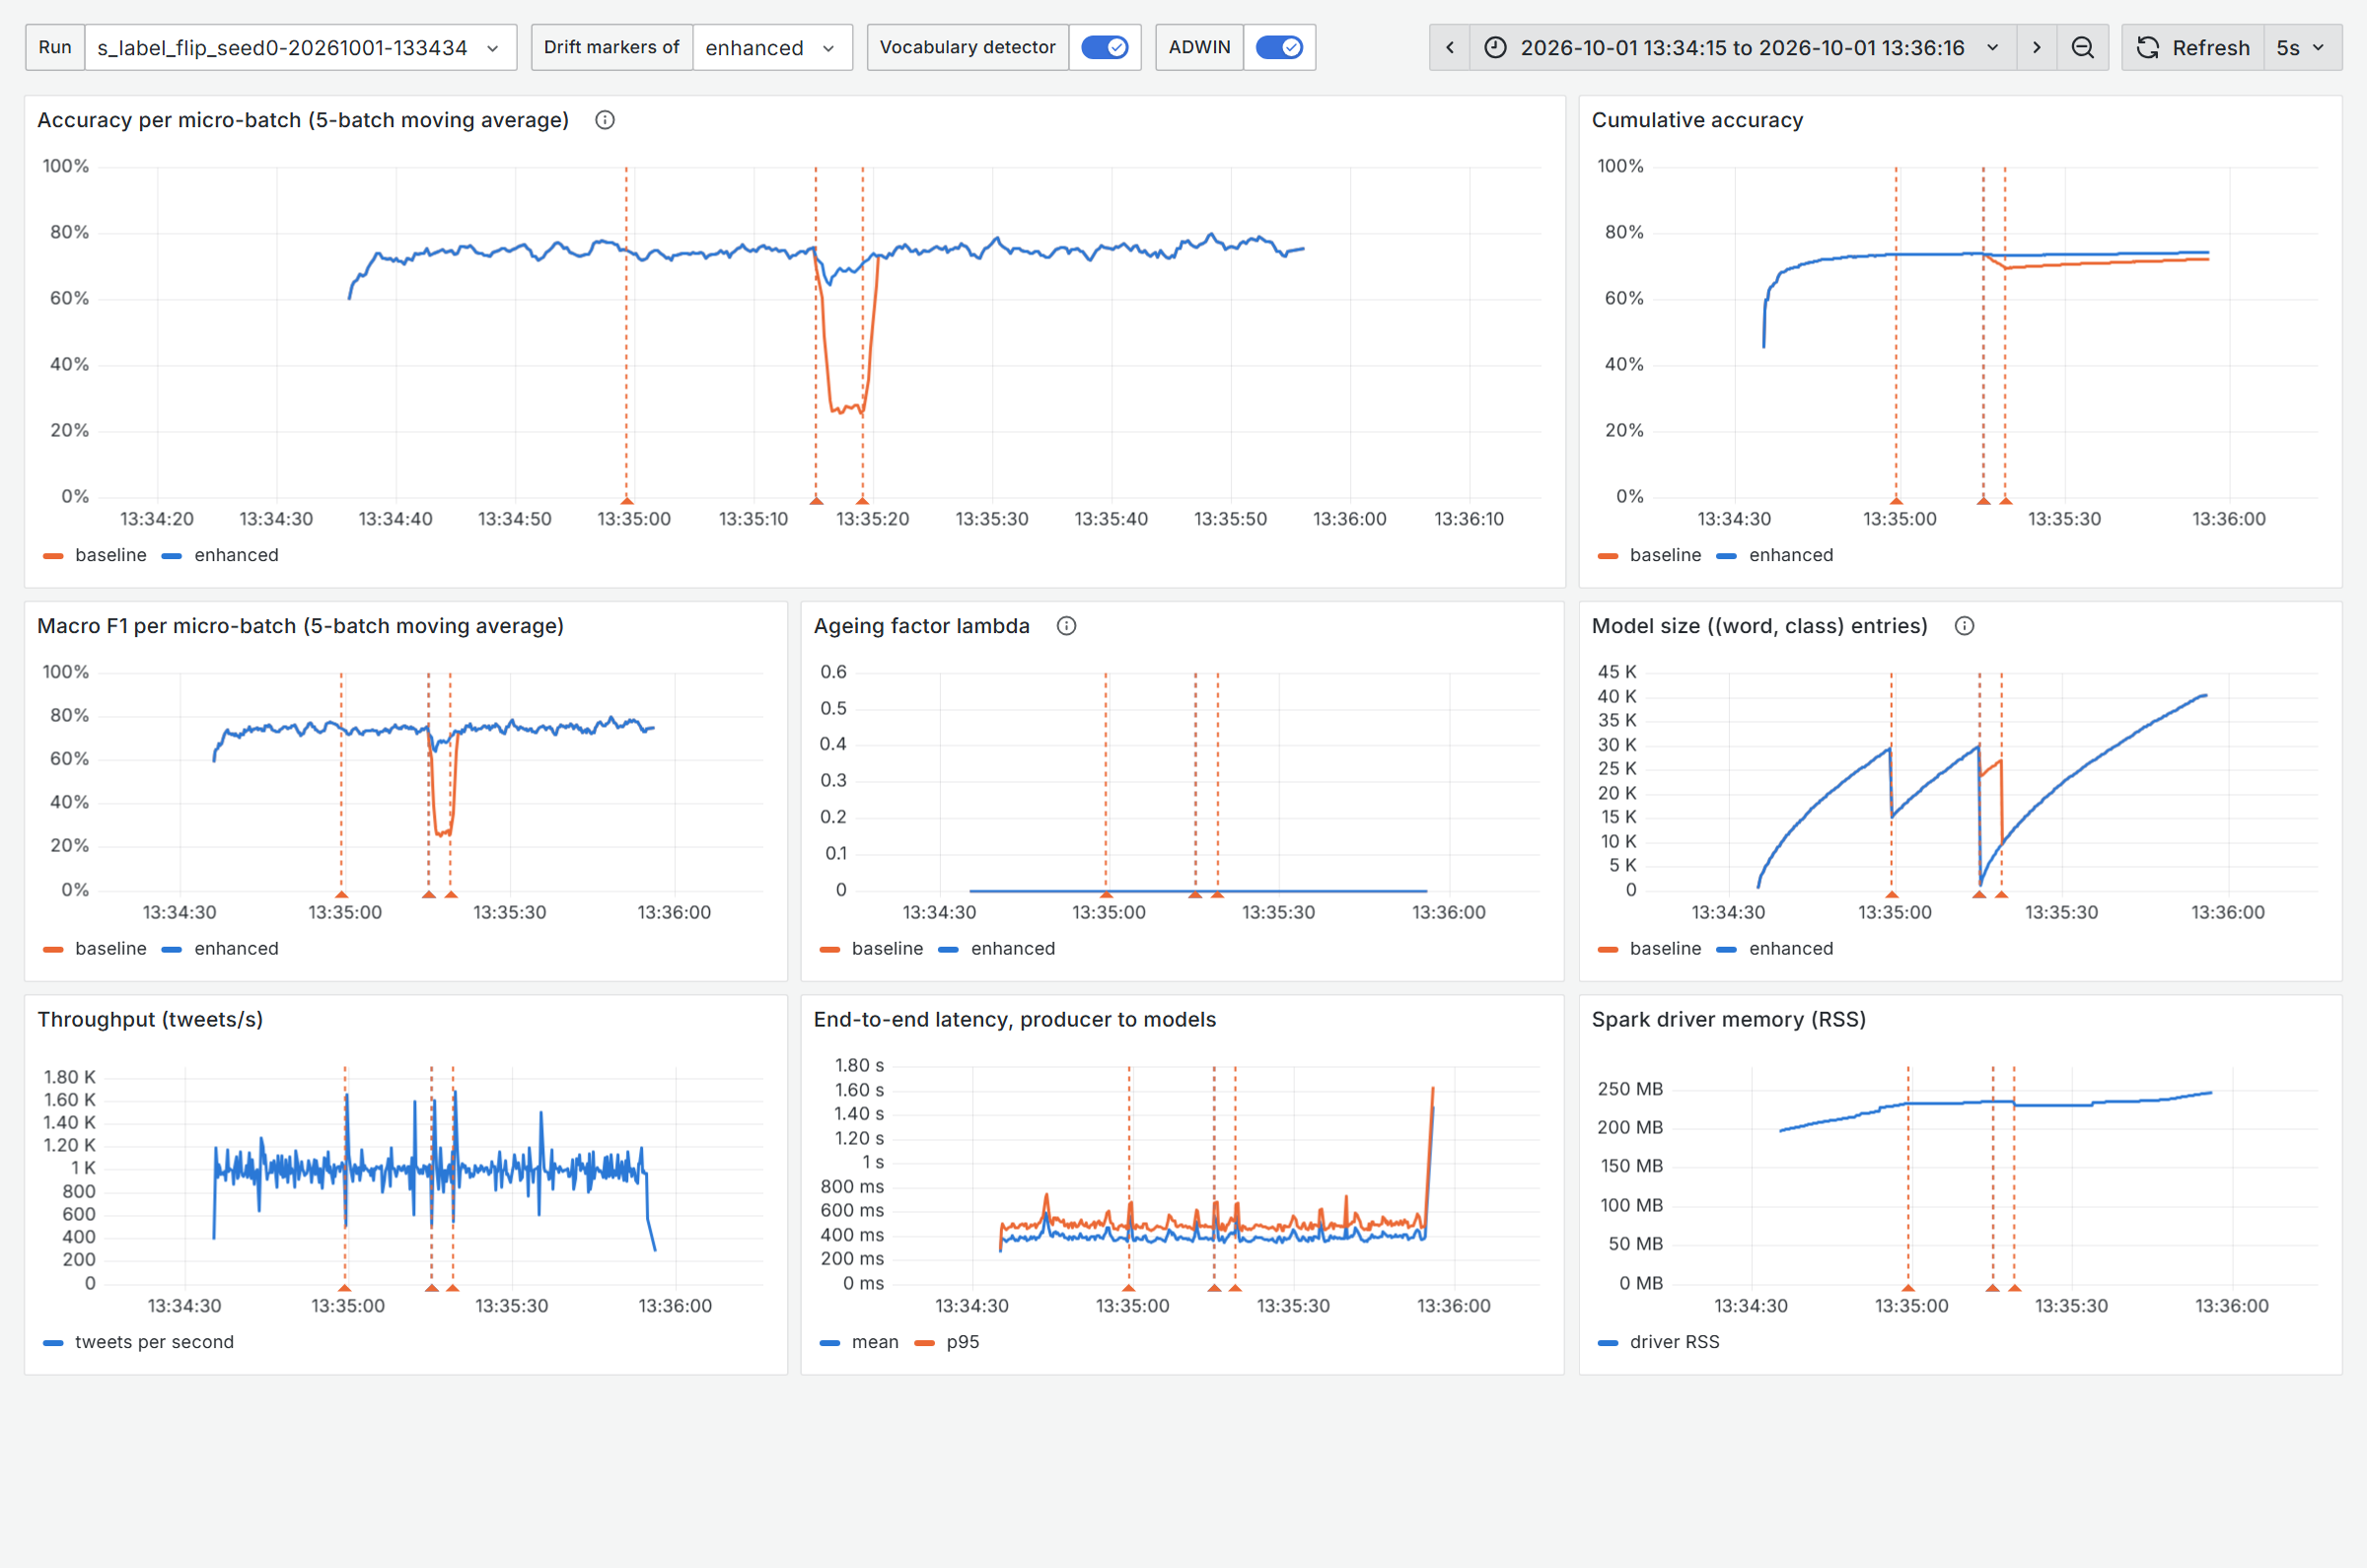
\includegraphics[width=\textwidth]{grafana_label_flip.png}
\column{0.42\textwidth}
\small
\begin{itemize}
\item live = offline: 72\% vs 74\% on the label flip
\item 2,000 tweets/s at 0.4\,s median latency (1k batches); 5,600 tweets/s with 5k batches
\item model time per 1k tweets: \bas{22.6\,ms} vs \enh{32.9\,ms}; Spark overhead \textasciitilde170\,ms per batch
\end{itemize}
\end{columns}
\end{frame}

\begin{frame}{Takeaways and limitations}
\begin{itemize}
\item Watch the \textbf{errors}, not only the \textbf{words}: ADWIN sees meaning drift the
  vocabulary detector misses or delays (\textasciitilde100$\times$ faster on the label flip).
\item The detectors are \textbf{complementary}: vocabulary $\to$ prior / topic shifts; ADWIN $\to$
  $P(y|X)$ changes.
\item Virtual drift barely hurts MNB; $\lambda$ strategies depend on the time scale, rebuild does
  not; naive Bayes cannot learn a topic-specific flip (\textasciitilde64\% ceiling).
\item \textbf{Limitations:} noisy emoticon labels, synthetic drifts, DS1/DS2 ground truth only has
  designed drift points, sequential model on the Spark driver, 2009 data.
\end{itemize}
\end{frame}

\begin{frame}[c]
\centering\Large Thank you --- questions?\\[1em]
\normalsize Code, data scripts, results: \texttt{github.com/CASPER0022/Drift-Aware-Sentiment-Stream}
\end{frame}

\appendix
\begin{frame}{Backup: Q\&A}
\small
\begin{description}
\item[Why MNB?] The base paper's model; one pass, $O(|d|)$ per tweet, interpretable counts that
  ageing can weight; lets us change \emph{only} the detector.
\item[Why ADWIN, not DDM or Page-Hinkley?] Parameter-light (one $\delta$), no fixed window,
  guarantees on false positives / negatives, and it reports a window width we reuse as the
  rebuild set.
\item[How is detection delay measured?] First detection the model acted on inside
  $[p, p+T)$ after a known drift point $p$ ($T$ = 10k scenarios, 50k real); others are false
  alarms.
\item[Why Spark if the model is sequential?] Spark scales ingestion, parsing and tokenisation and
  gives exactly-once micro-batches from Kafka; the stateful model runs on the driver. Keyed
  state per entity would let Spark partition the model too.
\item[How were the drifts made?] Real Sentiment140 tweets, topic pools by keywords, balanced per
  class, re-timestamped into an 80k stream with the drift at a known instance (Costa et al.).
\end{description}
\end{frame}

\end{document}
